\documentclass[14pt]{beamer}
\usetheme{Warsaw}
\usepackage[utf8]{vietnam}
\usepackage{ragged2e}
\usepackage{framed}
\usepackage{boxedminipage}
\useoutertheme{shadow}
%\setbeamertemplate{navigation symbols}{}
\setbeamertemplate{frametitle}[default][center]
\setbeamertemplate{headline}
{
  \leavevmode%
  \hbox{%
  \begin{beamercolorbox}[wd=.5\paperwidth,ht=2.65ex,dp=1.5ex,right]{section in head/foot}%
    \usebeamerfont{section in head/foot}\insertsectionhead\hspace*{2ex}
  \end{beamercolorbox}%
  \begin{beamercolorbox}[wd=.5\paperwidth,ht=2.65ex,dp=1.5ex,left]{subsection in head/foot}%
    \usebeamerfont{subsection in head/foot}\hspace*{2ex}\insertsubsectionhead
  \end{beamercolorbox}}%
  \vskip0pt%
}

\newcommand*\oldmacro{}
\let\oldmacro\insertshortauthor
\renewcommand*\insertshortauthor{
  \leftskip=.3cm
  \insertframenumber\,/\,\inserttotalframenumber\hfill\oldmacro
}

\usepackage{graphicx}
\usepackage{hyperref}
\hypersetup{
  colorlinks        = false,
  bookmarksnumbered = true,
  unicode           = true,
  pdfauthor         = {Duong Tien Thuan - 50TH2 - 0851061294},
  pdftitle          = {TIEP CAN SYSTEM AUTOMATION CHO HA TANG SAN PHAM CONG NGHE},
  pdfsubject        = {DO AN TOT NGHIEP - CSE - WRU},
  pdfcreator        = {Thuan Duong <thuandt26@gmail.com>},
  pdfproducer       = {pdflatex}
}

\title[Tiếp cận System Automation cho hạ tầng sản phẩm công nghệ]{Tiếp cận System Automation cho hạ tầng sản phẩm công nghệ}
\author[Dương Tiến Thuận - 50TH2]{SV: Dương Tiến Thuận - 50TH2\\GVHD: Th.S Nguyễn Nam Hưng}

\begin{document}

\AtBeginSection[]
{
  \begin{frame}
    \frametitle{Nội dung}
    \tableofcontents[currentsection]
  \end{frame}
}

\begin{frame}{BẢO VỆ ĐỒ ÁN TỐT NGHIỆP}
    \titlepage
\end{frame}

\begin{frame}
  \frametitle{Nội dung}
  \tableofcontents
\end{frame}

\section{Tổng quan}
\begin{frame}{System Automation}
  \begin{alertblock}\justifying
    \Large Tự động hóa các công việc thủ công lặp đi lặp lại đối với người quản trị hệ thống: cài đặt - cấu hình máy chủ, triển khai ứng dụng ..
  \end{alertblock}
\end{frame}

\begin{frame}{Tại sao cần phải tự động hóa?}
  \begin{alertblock}\justifying
    \begin{itemize}
      \item \Large Giảm thiểu sự nhàm chán
      \item \Large Tăng hiệu quả công việc
      \item \Large Giảm thiểu sai sót không đáng có do yếu tố con người
    \end{itemize}
  \end{alertblock}
\end{frame}

\begin{frame}{Sự cần thiết của các công cụ tự động hóa}
  \begin{itemize}
    \item Các kịch bản tùy chỉnh thường phức tạp và không có tài liệu kèm theo.
    \pause
    \item Các kịch bản tùy chỉnh ít có khả năng mở rộng hoặc sử dụng lại.
    \pause
    \item Sự gia tăng số lượng máy chủ phải quản lý do sự phát triển của công nghệ điện toán đám mây.
  \end{itemize}
\end{frame}

\section{Các công cụ trong tự động hóa hệ thống}
\subsection{Puppet}
\subsubsection*{Tổng quan về Puppet}
\begin{frame}{Tổng quan về Puppet}
  \begin{itemize}
    \item \textbf{Puppet} là một phần mềm \textbf{Mã Nguồn Mở} được viết bằng Ruby.
    \pause
    \item \textbf{Puppet} được sử dụng rộng rãi bởi nhiều tập đoàn lớn: Google, Twitter .v.v
    \pause
    \item \textbf{Puppet} có khả năng quản lý số lượng máy chủ cực kì lớn.
    \pause
    \item \textbf{Puppet} có thể chạy trên rất nhiều các nền tảng khác nhau.
  \end{itemize}
\end{frame}

\subsubsection*{Kiến trúc hệ thống của Puppet}
\begin{frame}{Kiến trúc hệ thống của Puppet}
  \setlength{\topsep}{0pt}
  \begin{columns}
    \begin{column}{0.75\textwidth}
      \begin{center}
        \fbox{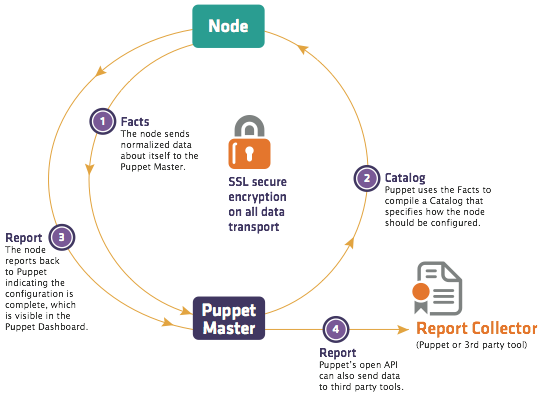
\includegraphics[width=\textwidth]{images/puppet_dataflow.png}}
      \end{center}
    \end{column}
    \hfill
    \pause
    \begin{column}{0.38\textwidth}
      \begin{scriptsize}
        \begin{itemize}
          \item \textbf{Agent}: Thực hiện những công việc mà Puppet Master yêu cầu.
          \pause
          \item \textbf{Puppet Master}: Máy chủ trung tâm.
          \pause
          \item \textbf{Facter}: Thu thập các thông tin cần thiết cho Puppet Master.
          \pause
          \item \textbf{Catalog}: Một đồ thị về các tài nguyên của máy chủ được quản lý và các rằng buộc giữa chúng.
          \pause
          \item \textbf{Reporting}: Các bản báo cáo.
        \end{itemize}
      \end{scriptsize}
    \end{column}
  \end{columns}
\end{frame}

\subsection{Chef}
\subsubsection*{Tổng quan về Chef}

\begin{frame}{Tổng quan về Chef}
\renewcommand{\baselinestretch}{1.50}\normalsize
  \begin{itemize}
    \item \textbf{Chef} là một phần mềm \textbf{Mã Nguồn Mở} được viết bằng Ruby.
    \pause
    \item \textbf{Chef} là một công cụ tự động hóa hệ thống và cơ sở hạ tầng điện toán đám mây.
    \pause
    \item \textbf{Chef} có khả năng triển khai các máy chủ hoặc các ứng dụng tới bất kì đâu.
  \end{itemize}
\renewcommand{\baselinestretch}{1.0}\normalsize
\end{frame}

\subsubsection*{Kiến trúc hệ thống của Chef}
\begin{frame}{Kiến trúc hệ thống của Chef}
  \setlength{\topsep}{0pt}
  \begin{columns}
    \begin{column}{0.75\textwidth}
      \begin{center}
        \fbox{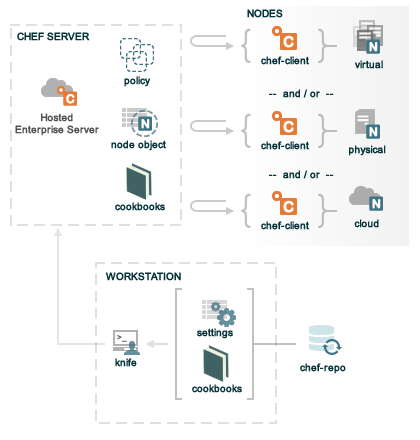
\includegraphics[width=0.85\textwidth]{images/chef_quick_overview.png}}
      \end{center}
    \end{column}
    \hfill
    \pause
    \begin{column}{0.38\textwidth}
      \begin{scriptsize}
        \begin{itemize}
          \item \textbf{Các nút}: máy chủ vật lý, máy chủ ảo hay máy chủ nền điện toán đám mây.
          \pause
          \item \textbf{Máy chủ}: trung tâm chứa dữ liệu cấu hình.
          \pause
          \item \textbf{Máy trạm}: nơi được cấu hình để chạy Knife, nơi lưu trữ chef-repo.
          \pause
          \item \textbf{Knife}: một công cụ dòng lệnh cung cấp giao diện tương tác giữa chef-repo với máy chủ hoặc máy trạm.
          \pause
          \item \textbf{Chef-repo}: nơi lưu trữ các đối tượng dữ liệu.
          \pause
          \item \textbf{Cookbook}: đơn vị cơ bản của Chef. Mỗi cookbook định nghĩa một kịch bản cấu hình.
        \end{itemize}
      \end{scriptsize}
    \end{column}
  \end{columns}
\end{frame}

\subsection{Ansible}
\subsubsection*{Tổng quan về Ansible}

\begin{frame}{Tổng quan về Ansible}
\renewcommand{\baselinestretch}{1.50}\normalsize
  \begin{itemize}
    \item \textbf{Ansible} là một công cụ tự động hóa \textbf{Mã Nguồn Mở} được viết bằng Python.
    \pause
    \item \textbf{Ansible} rất dễ học và sử dụng nhưng lại rất mạnh mẽ.
    \pause
    \item \textbf{Ansible} được thiết kế nhỏ gọn, tiện dụng, an toàn và có độ tin cậy cao.
  \end{itemize}
\renewcommand{\baselinestretch}{1.0}\normalsize
\end{frame}

\subsubsection*{Kiến trúc hệ thống của Ansible}
\begin{frame}{Kiến trúc hệ thống của Ansible}
  \setlength{\topsep}{0pt}
  \begin{columns}
    \begin{column}{0.75\textwidth}
      \begin{center}
        \fbox{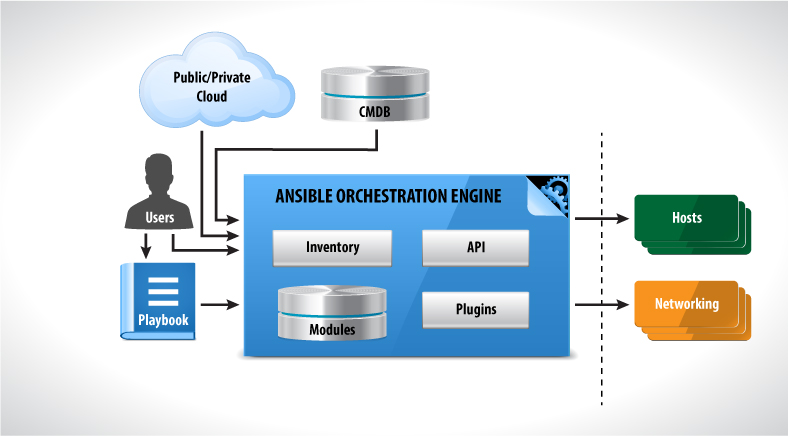
\includegraphics[width=\textwidth]{images/ansible_architect.jpg}}
      \end{center}
    \end{column}
    \hfill
    \pause
    \begin{column}{0.38\textwidth}
      \begin{scriptsize}
        \begin{itemize}
          \item \textbf{Modules}: Ansible có rất sẵn các module phục vụ hầu hết các công việc cơ bản của ngành IT.
          \pause
          \item \textbf{Plugins}: Ansible có rất nhiều các thành phần để chúng ta có thể tích hợp thêm những thứ cần thiết.
          \pause
          \item \textbf{Playbooks}: là tập hợp những cấu hình cụ thể thực hiện một số các công việc nhất định.
        \end{itemize}
      \end{scriptsize}
    \end{column}
  \end{columns}
\end{frame}

\section{Triển khai thực nghiệm}
\subsection{Bài toán}
\begin{frame}{Bài toán}
\renewcommand{\baselinestretch}{1.50}\normalsize
  \begin{alertblock}\justifying
    \emph{\textbf{"Viết công cụ tự động tạo ra một máy chủ trên nền điện toán đám mây Google Compute Engine (GCE). Sau đó tự động cài đặt và cấu hình hệ thống LAMP; cùng với đó là tự động triển khai CMS Wordpress phiên bản mới nhất lên trên máy chủ vừa tạo."}}
  \end{alertblock}
\renewcommand{\baselinestretch}{1.0}\normalsize
\end{frame}

\subsection{Phân tích}
\subsubsection*{Lựa chọn công cụ}
\begin{frame}{Lựa chọn công cụ}
\renewcommand{\baselinestretch}{1.50}\normalsize
  Ansible được chọn vì những lý do sau:
  \begin{itemize}
    \item Ansible rất dễ học và sử dụng.
    \pause
    \item Ansible được viết bằng Python.
    \pause
    \item Ansible phù hợp với tư duy của người quản trị hệ thống.
  \end{itemize}
\renewcommand{\baselinestretch}{1.0}\normalsize
\end{frame}


\begin{frame}{Phân tích}
\renewcommand{\baselinestretch}{1.50}\normalsize
  Những công việc cần phải thực hiện:
  \begin{itemize}
    \item Tạo máy chủ ảo trên hệ thống GCE.
    \pause
    \item Cài đặt và cấu hình LAMP.
    \pause
    \item Triển khai ứng dụng Wordpress CMS.
  \end{itemize}
\renewcommand{\baselinestretch}{1.0}\normalsize
\end{frame}

\subsection{Triển khai}
\begin{frame}{Viết các playbook cho Ansible}
  \begin{itemize}
  \item playbook gce
  \item playbook mysql
  \item playbook nginx
  \item playbook wordpress
  \end{itemize}
\end{frame}

\section{Demo}
\begin{frame}
  \begin{center}
  \fbox{
\includegraphics[width=0.7\textwidth]{images/demo.png}}
  \end{center}
\end{frame}

\section*{}
\begin{frame}
  \begin{center}
    \Huge Questions?
  \end{center}
\end{frame}

\section*{}
\begin{frame}
    \begin{center}
      \Huge Cám ơn mọi người đã lắng nghe!
    \end{center}
\end{frame}

\end{document}
